% Options for packages loaded elsewhere
\PassOptionsToPackage{unicode}{hyperref}
\PassOptionsToPackage{hyphens}{url}
%
\documentclass[
]{book}
\usepackage{amsmath,amssymb}
\usepackage{lmodern}
\usepackage{iftex}
\ifPDFTeX
  \usepackage[T1]{fontenc}
  \usepackage[utf8]{inputenc}
  \usepackage{textcomp} % provide euro and other symbols
\else % if luatex or xetex
  \usepackage{unicode-math}
  \defaultfontfeatures{Scale=MatchLowercase}
  \defaultfontfeatures[\rmfamily]{Ligatures=TeX,Scale=1}
\fi
% Use upquote if available, for straight quotes in verbatim environments
\IfFileExists{upquote.sty}{\usepackage{upquote}}{}
\IfFileExists{microtype.sty}{% use microtype if available
  \usepackage[]{microtype}
  \UseMicrotypeSet[protrusion]{basicmath} % disable protrusion for tt fonts
}{}
\makeatletter
\@ifundefined{KOMAClassName}{% if non-KOMA class
  \IfFileExists{parskip.sty}{%
    \usepackage{parskip}
  }{% else
    \setlength{\parindent}{0pt}
    \setlength{\parskip}{6pt plus 2pt minus 1pt}}
}{% if KOMA class
  \KOMAoptions{parskip=half}}
\makeatother
\usepackage{xcolor}
\usepackage{color}
\usepackage{fancyvrb}
\newcommand{\VerbBar}{|}
\newcommand{\VERB}{\Verb[commandchars=\\\{\}]}
\DefineVerbatimEnvironment{Highlighting}{Verbatim}{commandchars=\\\{\}}
% Add ',fontsize=\small' for more characters per line
\usepackage{framed}
\definecolor{shadecolor}{RGB}{248,248,248}
\newenvironment{Shaded}{\begin{snugshade}}{\end{snugshade}}
\newcommand{\AlertTok}[1]{\textcolor[rgb]{0.94,0.16,0.16}{#1}}
\newcommand{\AnnotationTok}[1]{\textcolor[rgb]{0.56,0.35,0.01}{\textbf{\textit{#1}}}}
\newcommand{\AttributeTok}[1]{\textcolor[rgb]{0.77,0.63,0.00}{#1}}
\newcommand{\BaseNTok}[1]{\textcolor[rgb]{0.00,0.00,0.81}{#1}}
\newcommand{\BuiltInTok}[1]{#1}
\newcommand{\CharTok}[1]{\textcolor[rgb]{0.31,0.60,0.02}{#1}}
\newcommand{\CommentTok}[1]{\textcolor[rgb]{0.56,0.35,0.01}{\textit{#1}}}
\newcommand{\CommentVarTok}[1]{\textcolor[rgb]{0.56,0.35,0.01}{\textbf{\textit{#1}}}}
\newcommand{\ConstantTok}[1]{\textcolor[rgb]{0.00,0.00,0.00}{#1}}
\newcommand{\ControlFlowTok}[1]{\textcolor[rgb]{0.13,0.29,0.53}{\textbf{#1}}}
\newcommand{\DataTypeTok}[1]{\textcolor[rgb]{0.13,0.29,0.53}{#1}}
\newcommand{\DecValTok}[1]{\textcolor[rgb]{0.00,0.00,0.81}{#1}}
\newcommand{\DocumentationTok}[1]{\textcolor[rgb]{0.56,0.35,0.01}{\textbf{\textit{#1}}}}
\newcommand{\ErrorTok}[1]{\textcolor[rgb]{0.64,0.00,0.00}{\textbf{#1}}}
\newcommand{\ExtensionTok}[1]{#1}
\newcommand{\FloatTok}[1]{\textcolor[rgb]{0.00,0.00,0.81}{#1}}
\newcommand{\FunctionTok}[1]{\textcolor[rgb]{0.00,0.00,0.00}{#1}}
\newcommand{\ImportTok}[1]{#1}
\newcommand{\InformationTok}[1]{\textcolor[rgb]{0.56,0.35,0.01}{\textbf{\textit{#1}}}}
\newcommand{\KeywordTok}[1]{\textcolor[rgb]{0.13,0.29,0.53}{\textbf{#1}}}
\newcommand{\NormalTok}[1]{#1}
\newcommand{\OperatorTok}[1]{\textcolor[rgb]{0.81,0.36,0.00}{\textbf{#1}}}
\newcommand{\OtherTok}[1]{\textcolor[rgb]{0.56,0.35,0.01}{#1}}
\newcommand{\PreprocessorTok}[1]{\textcolor[rgb]{0.56,0.35,0.01}{\textit{#1}}}
\newcommand{\RegionMarkerTok}[1]{#1}
\newcommand{\SpecialCharTok}[1]{\textcolor[rgb]{0.00,0.00,0.00}{#1}}
\newcommand{\SpecialStringTok}[1]{\textcolor[rgb]{0.31,0.60,0.02}{#1}}
\newcommand{\StringTok}[1]{\textcolor[rgb]{0.31,0.60,0.02}{#1}}
\newcommand{\VariableTok}[1]{\textcolor[rgb]{0.00,0.00,0.00}{#1}}
\newcommand{\VerbatimStringTok}[1]{\textcolor[rgb]{0.31,0.60,0.02}{#1}}
\newcommand{\WarningTok}[1]{\textcolor[rgb]{0.56,0.35,0.01}{\textbf{\textit{#1}}}}
\usepackage{longtable,booktabs,array}
\usepackage{calc} % for calculating minipage widths
% Correct order of tables after \paragraph or \subparagraph
\usepackage{etoolbox}
\makeatletter
\patchcmd\longtable{\par}{\if@noskipsec\mbox{}\fi\par}{}{}
\makeatother
% Allow footnotes in longtable head/foot
\IfFileExists{footnotehyper.sty}{\usepackage{footnotehyper}}{\usepackage{footnote}}
\makesavenoteenv{longtable}
\usepackage{graphicx}
\makeatletter
\def\maxwidth{\ifdim\Gin@nat@width>\linewidth\linewidth\else\Gin@nat@width\fi}
\def\maxheight{\ifdim\Gin@nat@height>\textheight\textheight\else\Gin@nat@height\fi}
\makeatother
% Scale images if necessary, so that they will not overflow the page
% margins by default, and it is still possible to overwrite the defaults
% using explicit options in \includegraphics[width, height, ...]{}
\setkeys{Gin}{width=\maxwidth,height=\maxheight,keepaspectratio}
% Set default figure placement to htbp
\makeatletter
\def\fps@figure{htbp}
\makeatother
\setlength{\emergencystretch}{3em} % prevent overfull lines
\providecommand{\tightlist}{%
  \setlength{\itemsep}{0pt}\setlength{\parskip}{0pt}}
\setcounter{secnumdepth}{5}
\usepackage{booktabs}
\usepackage[finnish]{babel}
\usepackage{amsthm}
\usepackage{amsmath}
\makeatletter
\def\thm@space@setup{%
  \thm@preskip=8pt plus 2pt minus 4pt
  \thm@postskip=\thm@preskip
}
\makeatother
\ifLuaTeX
  \usepackage{selnolig}  % disable illegal ligatures
\fi
\usepackage[]{natbib}
\bibliographystyle{apalike}
\IfFileExists{bookmark.sty}{\usepackage{bookmark}}{\usepackage{hyperref}}
\IfFileExists{xurl.sty}{\usepackage{xurl}}{} % add URL line breaks if available
\urlstyle{same} % disable monospaced font for URLs
\hypersetup{
  pdftitle={Esimerkkikirja},
  pdfauthor={MathHub Tiimi},
  hidelinks,
  pdfcreator={LaTeX via pandoc}}

\title{Esimerkkikirja}
\author{MathHub Tiimi}
\date{2023-05-30}

\usepackage{amsthm}
\newtheorem{theorem}{Teoreema}[chapter]
\newtheorem{lemma}{Lemma}[chapter]
\newtheorem{corollary}{Korollaari}[chapter]
\newtheorem{proposition}{Propositio}[chapter]
\newtheorem{conjecture}{Konjektuuri}[chapter]
\theoremstyle{definition}
\newtheorem{definition}{Määritelmä}[chapter]
\theoremstyle{definition}
\newtheorem{example}{Esimerkki}[chapter]
\theoremstyle{definition}
\newtheorem{exercise}{Tehtävä}[chapter]
\theoremstyle{definition}
\newtheorem{hypothesis}{Hypoteesi}[chapter]
\theoremstyle{remark}
\newtheorem*{remark}{Huomio}
\newtheorem*{solution}{Ratkaisu}
\begin{document}
\maketitle

{
\setcounter{tocdepth}{1}
\tableofcontents
}
\hypertarget{asennus}{%
\chapter{Asennus}\label{asennus}}

\emph{Index} on ensimmäinen sivu joka kirjasta tulee näkyviin.

Pandoc's Markdown toimii kirjassa, esimerkiksi: \(a^2 + b^2 = c^2\).

Jokainen .Rmd tiedosto sisältää yhden kirjan kappaleen, ja kappale muodostetaan ensimmäisen tason \texttt{\#} heading-merkinnällä.

\begin{enumerate}
\def\labelenumi{\arabic{enumi}.}
\tightlist
\item
  Päästäksesi alkuun kirjan muokkaamisessa, seuraavaksi asenna \textbf{bookdown} paketti. Voit asentaa paketin RStudiossa seuraavalla komennolla:
\end{enumerate}

\begin{Shaded}
\begin{Highlighting}[]
\FunctionTok{install.packages}\NormalTok{(}\StringTok{"bookdown"}\NormalTok{)}
\end{Highlighting}
\end{Shaded}

\begin{enumerate}
\def\labelenumi{\arabic{enumi}.}
\setcounter{enumi}{1}
\tightlist
\item
  Jotta saat PDF, .epub ja .tex -versiot kirjasta tuotettua, asenna TinyTex ajamalla seuraava komento:
\end{enumerate}

\begin{Shaded}
\begin{Highlighting}[]
\NormalTok{tinytex}\SpecialCharTok{::}\FunctionTok{install\_tinytex}\NormalTok{()}
\end{Highlighting}
\end{Shaded}

\begin{enumerate}
\def\labelenumi{\arabic{enumi}.}
\setcounter{enumi}{2}
\tightlist
\item
  Seuraavaksi asenna \texttt{xml2} ja \texttt{downlit}
\end{enumerate}

\begin{Shaded}
\begin{Highlighting}[]
\FunctionTok{install.packages}\NormalTok{(}\StringTok{"xml2"}\NormalTok{)}
\FunctionTok{install.packages}\NormalTok{(}\StringTok{"downlit"}\NormalTok{)}
\end{Highlighting}
\end{Shaded}

\begin{enumerate}
\def\labelenumi{\arabic{enumi}.}
\setcounter{enumi}{3}
\tightlist
\item
  Voit koota kirjan painamalla RStudiossa oikealla ylhäällä \texttt{Build}-välilehdeltä ``Build Book'' nappia. Tämä rakentaa sekä html, PDF, epub ja tex -versiot. HTML versio kirjasta löytyy \_book -kansiosta.
\end{enumerate}

\hypertarget{alku}{%
\chapter{Alku}\label{alku}}

Ristiviittauksia varten kappaleet ja otsikot voi nimetä \texttt{\{\#label\}} merkinnällä niiden jälkeen. Sen jälkeen voimme referoida kappaleeseen näin: \ref{alku}.

Kaaviot ja data kuvateksteineen voidaan tehdä \texttt{figure} ja \texttt{table} komennoilla.

\begin{Shaded}
\begin{Highlighting}[]
\FunctionTok{par}\NormalTok{(}\AttributeTok{mar =} \FunctionTok{c}\NormalTok{(}\DecValTok{4}\NormalTok{, }\DecValTok{4}\NormalTok{, .}\DecValTok{1}\NormalTok{, .}\DecValTok{1}\NormalTok{))}
\FunctionTok{plot}\NormalTok{(pressure, }\AttributeTok{type =} \StringTok{\textquotesingle{}b\textquotesingle{}}\NormalTok{, }\AttributeTok{pch =} \DecValTok{19}\NormalTok{)}
\end{Highlighting}
\end{Shaded}

\begin{figure}

{\centering 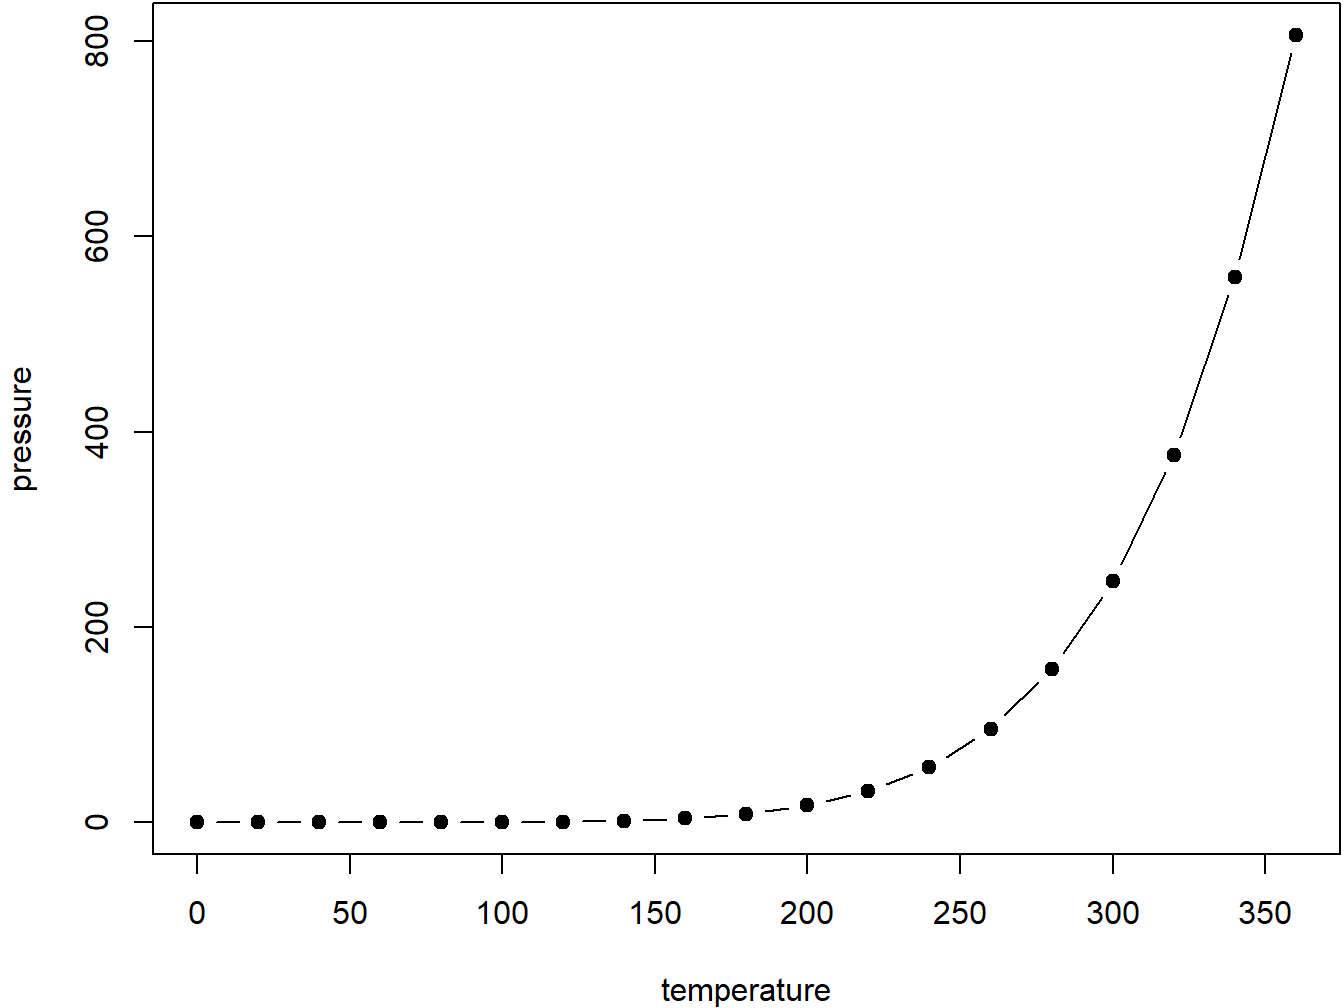
\includegraphics[width=0.8\linewidth]{bookdown-demo_files/figure-latex/nice-fig-1} 

}

\caption{Esimerkkikaavio}\label{fig:nice-fig}
\end{figure}

Kuvaa voidaan referoida \texttt{fig:} prefixillä, kuten Kuva \ref{fig:nice-fig} ja taulukkoon \texttt{tab:} prefixillä, kuten Taulukko \ref{tab:nice-tab}.

\begin{Shaded}
\begin{Highlighting}[]
\NormalTok{knitr}\SpecialCharTok{::}\FunctionTok{kable}\NormalTok{(}
  \FunctionTok{head}\NormalTok{(iris, }\DecValTok{20}\NormalTok{), }\AttributeTok{caption =} \StringTok{\textquotesingle{}Tietotaulukko\textquotesingle{}}\NormalTok{,}
  \AttributeTok{booktabs =} \ConstantTok{TRUE}
\NormalTok{)}
\end{Highlighting}
\end{Shaded}

\begin{table}

\caption{\label{tab:nice-tab}Tietotaulukko}
\centering
\begin{tabular}[t]{rrrrl}
\toprule
Sepal.Length & Sepal.Width & Petal.Length & Petal.Width & Species\\
\midrule
5.1 & 3.5 & 1.4 & 0.2 & setosa\\
4.9 & 3.0 & 1.4 & 0.2 & setosa\\
4.7 & 3.2 & 1.3 & 0.2 & setosa\\
4.6 & 3.1 & 1.5 & 0.2 & setosa\\
5.0 & 3.6 & 1.4 & 0.2 & setosa\\
\addlinespace
5.4 & 3.9 & 1.7 & 0.4 & setosa\\
4.6 & 3.4 & 1.4 & 0.3 & setosa\\
5.0 & 3.4 & 1.5 & 0.2 & setosa\\
4.4 & 2.9 & 1.4 & 0.2 & setosa\\
4.9 & 3.1 & 1.5 & 0.1 & setosa\\
\addlinespace
5.4 & 3.7 & 1.5 & 0.2 & setosa\\
4.8 & 3.4 & 1.6 & 0.2 & setosa\\
4.8 & 3.0 & 1.4 & 0.1 & setosa\\
4.3 & 3.0 & 1.1 & 0.1 & setosa\\
5.8 & 4.0 & 1.2 & 0.2 & setosa\\
\addlinespace
5.7 & 4.4 & 1.5 & 0.4 & setosa\\
5.4 & 3.9 & 1.3 & 0.4 & setosa\\
5.1 & 3.5 & 1.4 & 0.3 & setosa\\
5.7 & 3.8 & 1.7 & 0.3 & setosa\\
5.1 & 3.8 & 1.5 & 0.3 & setosa\\
\bottomrule
\end{tabular}
\end{table}

Sitaatit toimivat näin: Esimerkiksi, käytämme \textbf{bookdown} pakettia \citep{R-bookdown}.

Matemaattisia teoreemia ja todistuksia voi kirjata ylös

\begin{theorem}[Minun Teoreema]
\protect\hypertarget{thm:my-theorem}{}\label{thm:my-theorem}Olkoon \(a\) ja \(b\) sekä \(c\). Tällöin pätee
\begin{equation*}
  a-b=c
\end{equation*}
\end{theorem}

\begin{proof}
Todistus on triviaali.
\end{proof}

ja niihin voi viitata vastaavasti \texttt{thm:}prefixillä kuten Teoreema \ref{thm:my-theorem}. (Ei kuitenkaan ole vielä selvää, kuinka teoreema-ympäristöjen sisään voisi sisällyttää esim. kuvia)

Myös youtube upotuksia voi tehdä:

Ja myös geogebra appletteja:

\hypertarget{pythagoraan-lause}{%
\chapter{Pythagoraan lause}\label{pythagoraan-lause}}

Visa ja Fanny suunnitelevat ja koodaavat työkseen tietokonepelejä. He käyttävät tähän Unity-pelimoottoria. Pelimoottorissa pelimaailma esitetään rautalankamallina erilaisilla monikulmioilla, joista tärkein on kolmio.

\begin{figure}

{\centering 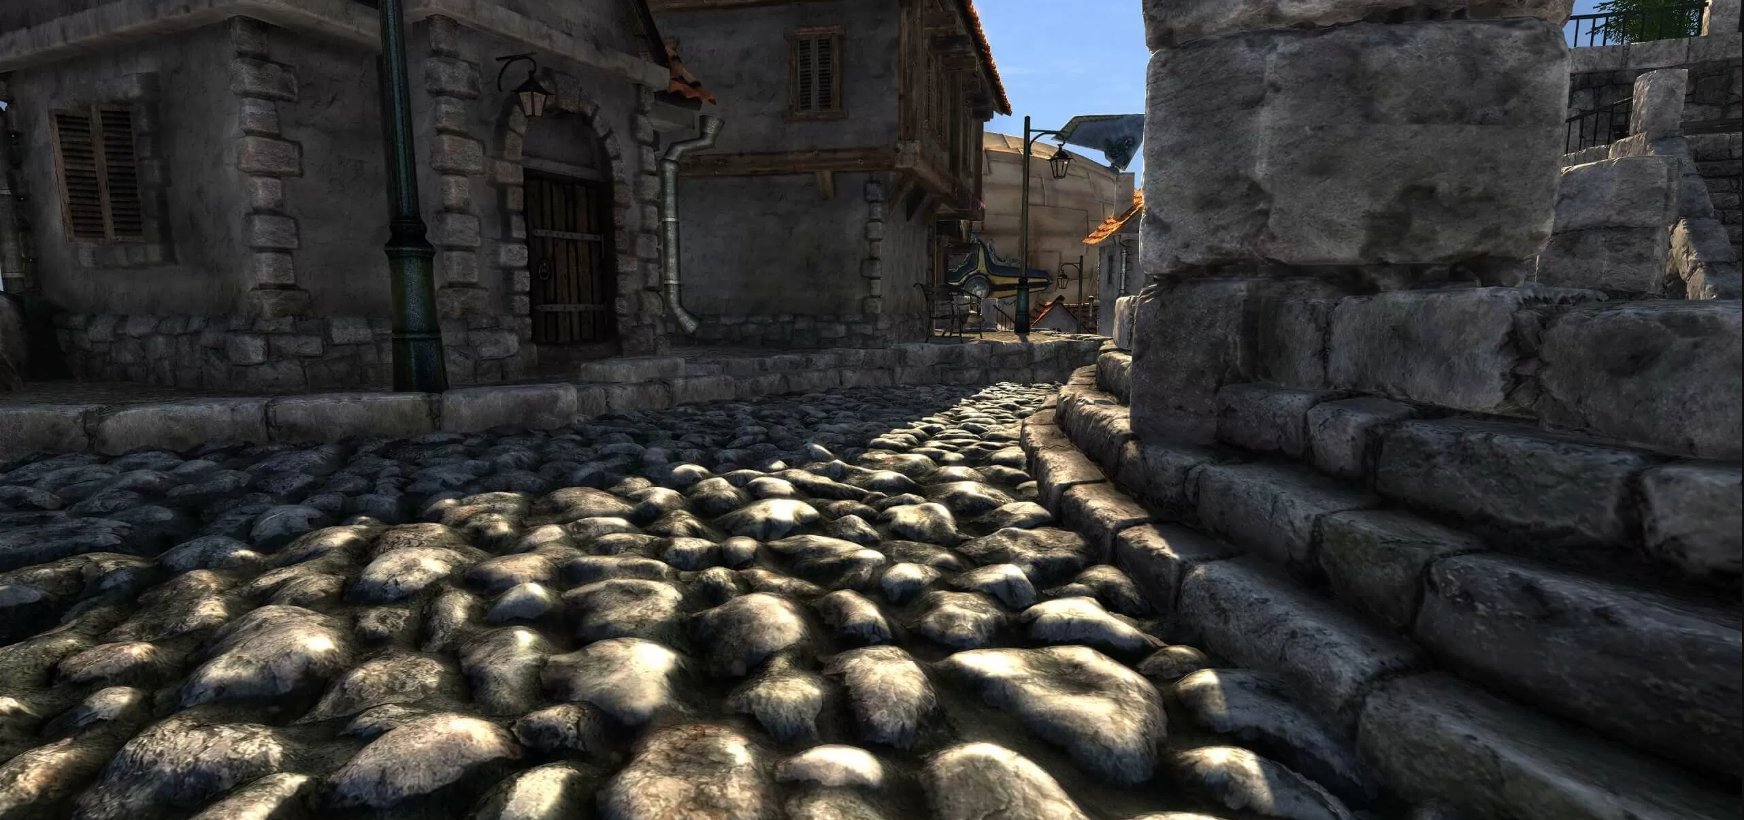
\includegraphics[width=0.8\linewidth,height=0.4\textheight]{img/renderoity} 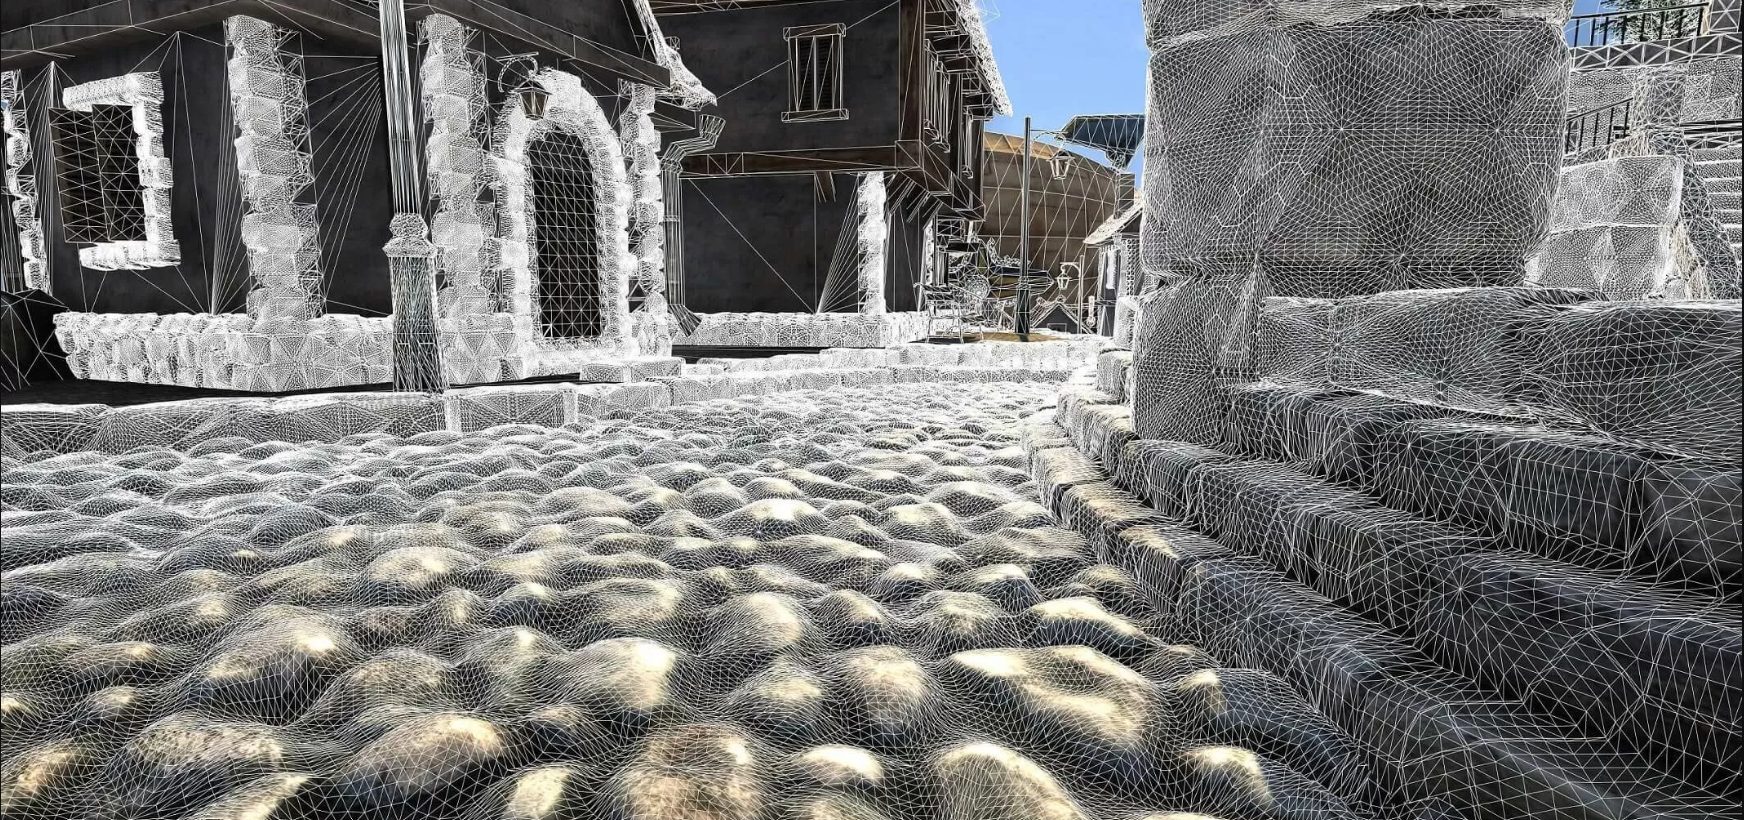
\includegraphics[width=0.8\linewidth,height=0.4\textheight]{img/rautalanka} 

}

\caption{Pelimaailma rakennetaan kolmioista}\label{fig:unnamed-chunk-7}
\end{figure}

Peleissä kolmioita käytetään määrittämään myös pelaajan etäisyys pelimaailman esineistä ja muodoista. Ensin pelaajan ja esineiden paikka kartalla määritetään koordinaateilla. Sitten koordinaattien avulla piirretään suorakulmainen kolmio kuvan \ref{fig:pelaaja-esine-kolmio} mukaisesti.

\begin{figure}

{\centering 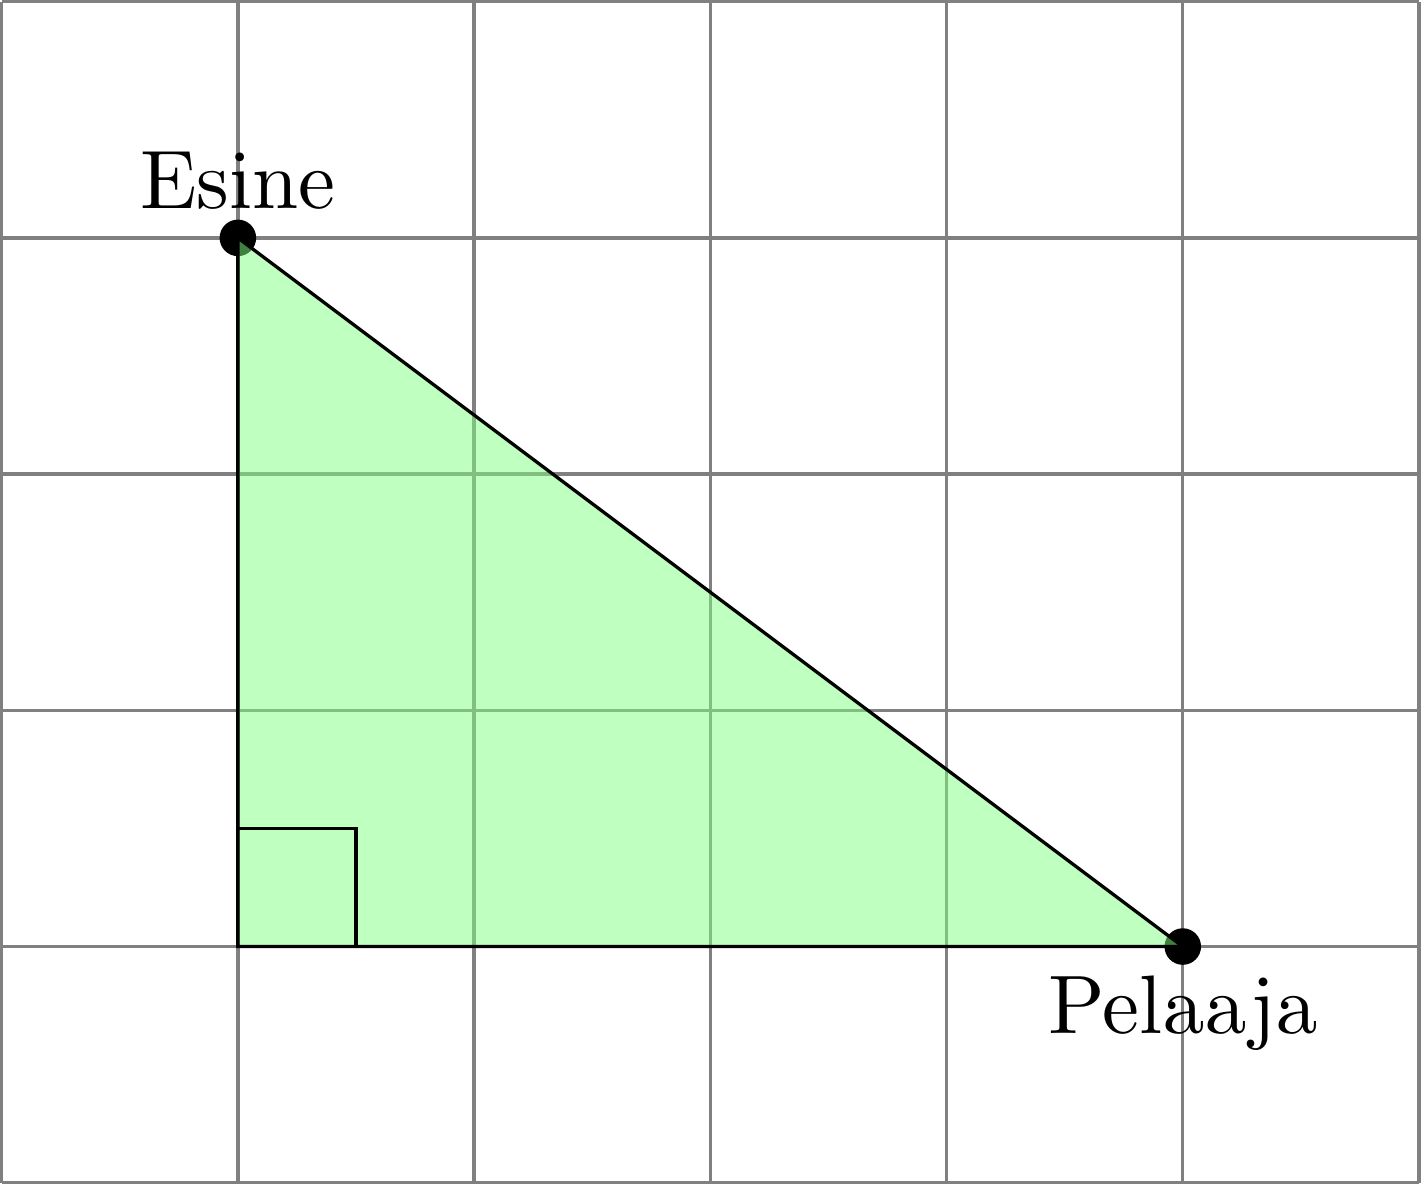
\includegraphics[width=0.4\linewidth,height=0.4\textheight]{img/pelaaja-esine} 

}

\caption{Pelaaja, esine ja suorakulmainen kolmio koordinaatistossa}\label{fig:pelaaja-esine-kolmio}
\end{figure}

Näin pelaajan ja esineen etäisyys saadaan selville laskemalla suorakulmaisen kolmion hypotenuusan pituus. Mutta kuinka hypotenuusan pituus lasketaan? Selvitetäänpä tämä mysteeri pohtimalla seuraavia kysymyksiä:

Huomataan, että sinisen neliön pinta-ala on yhtä suuri kuin vihreän kolmion kateettien neliöiden summa. Koska vihreän kolmion hypotenuusa on myös sinisen neliön sivu, voidaan todeta:

\textbf{Suorakulmaisen kolmion kateettien neliöiden summa on hypotenuusan neliö:}
\begin{align*}
  3^2+4^2=5^2
\end{align*}

\textbf{Suorakulmaisen kolmion hypotenuusan pituus on neliöjuuri kateettien neliöiden summasta:}
\begin{align*}
  5=\sqrt{3^2+4^2}
\end{align*}

Hieno havainto! Mutta päteekö tämä tulos kaikille suorakulmaisille kolmioille? Mitä tapahtuu, jos kateettien pituudet eivät olekaan 3 ja 4? Tutkitaan asiaa piirtämällä kuvaan \ref{fig:pythagoras-theorem} punainen nelio, neljä vihreää kolmiota ja sininen neliö uudestaan, mutta oletetaan kolmion kateettien pituuksiksi nyt \(a\) ja \(b\) sekä hypotenuusan pituudeksi \(c\). Lasketaan näillä tiedoilla myös eri väristen alueiden pinta-alat:

\begin{figure}

{\centering 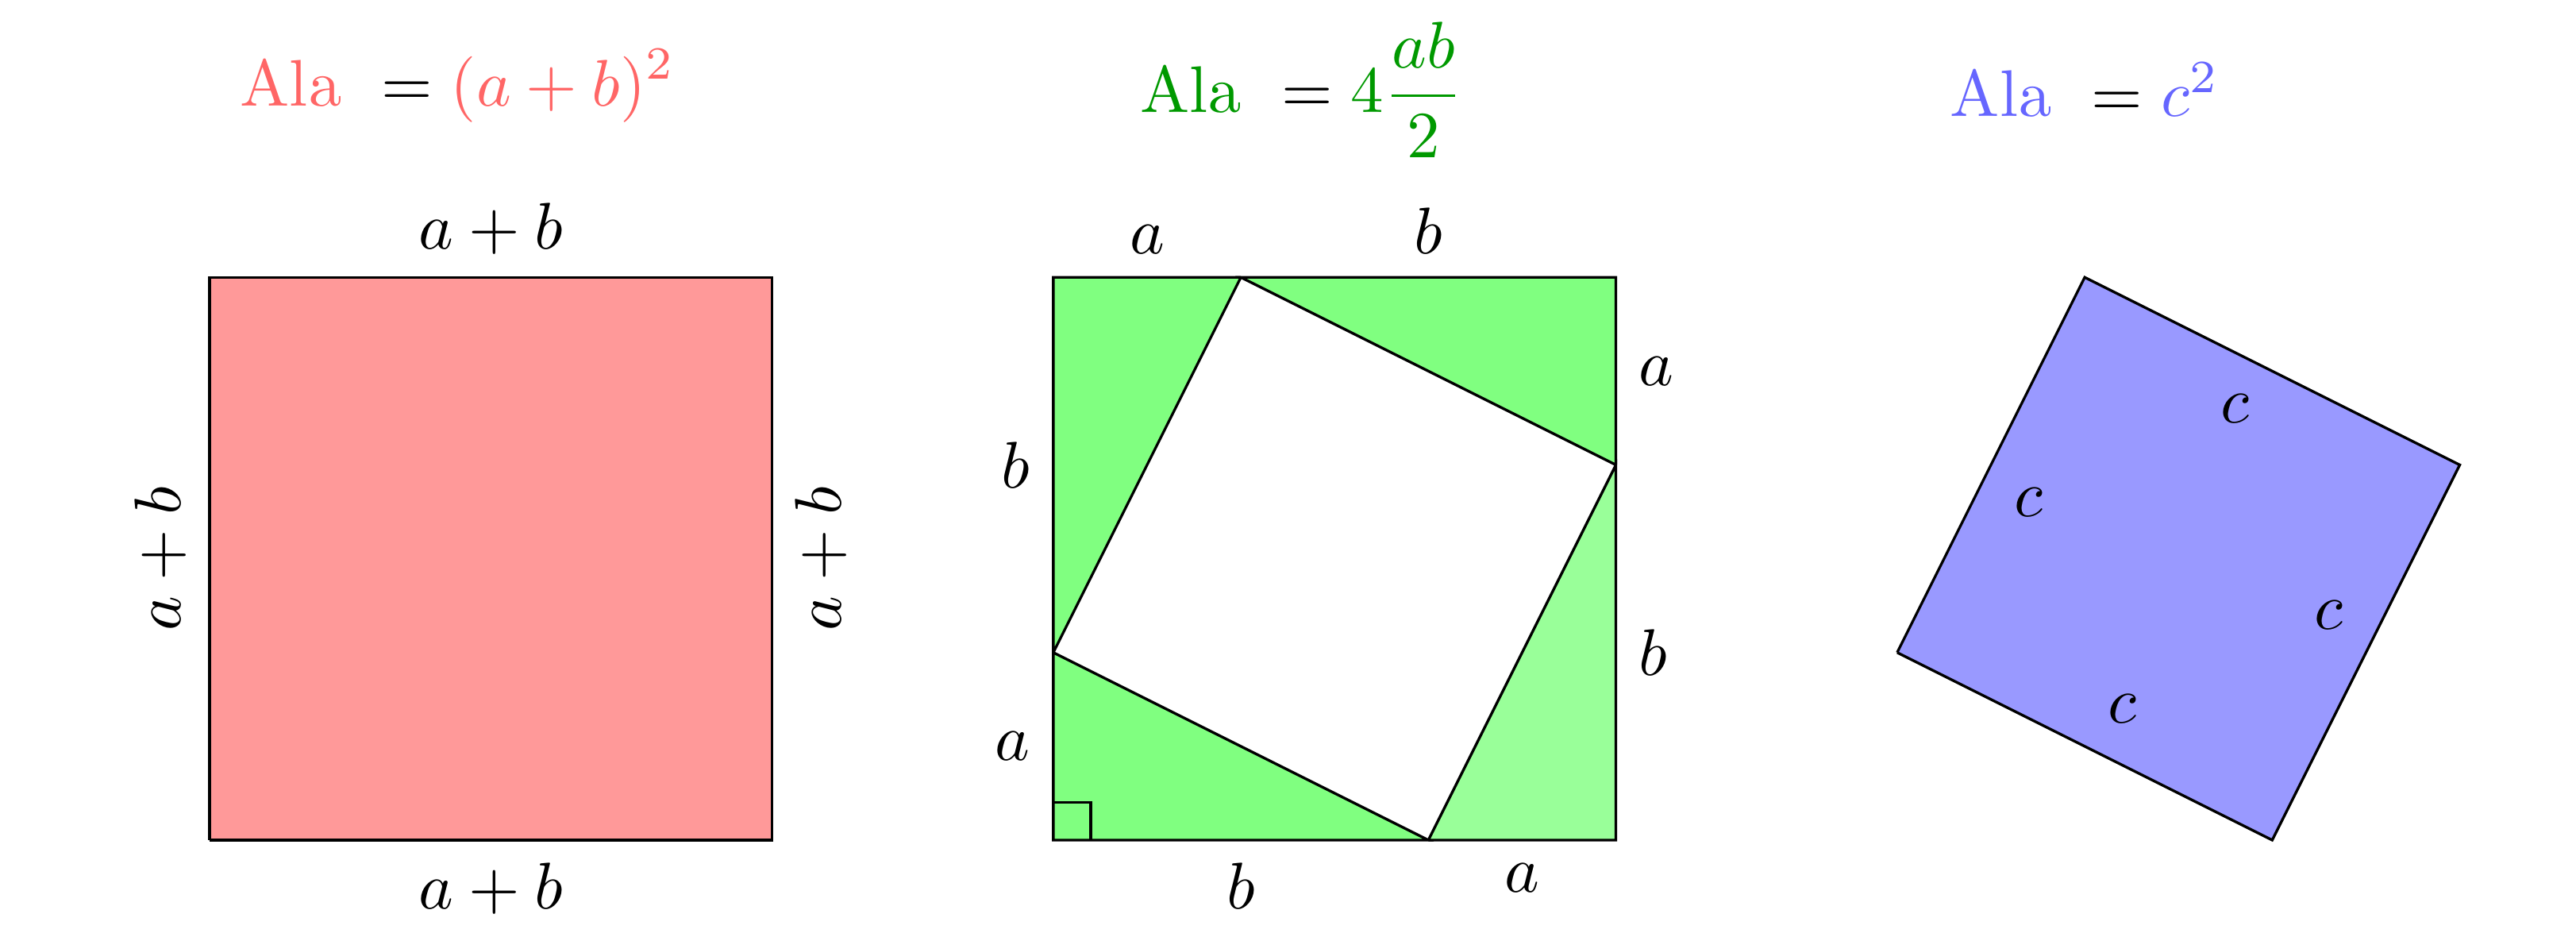
\includegraphics[width=1\linewidth,height=0.4\textheight]{img/pythagoraan-teoreema-todistus} 

}

\caption{Pinta-alojen laskeminen}\label{fig:pythagoras-theorem}
\end{figure}

Muistetaan, että sinisen neliön pinta-ala saadaan vähentämällä punaisen neliön pinta-alasta neljän vihreän kolmion yhteenlaskettu pinta-ala:
\begin{align*}
 \color{red}{\text{Punainen neliö }}- \color{green}{\text{ vihreät kolmiot }}&=\color{blue}{\text{ sininen neliö}},\\
  \color{red}{(a+b)^2} - \color{green}{4\frac{ab}{2}}&=\color{blue}{c^2},\\
  \color{red}{a^2+2ab+b^2} - \color{green}{2ab}&=\color{blue}{c^2}.
\end{align*}
Koska \(\color{red}{2ab} - \color{green}{2ab}=0\), saadaan lopulta tärkeä tulos:

\textbf{Pythagoraan lause:}

Olkoon suorakulmaisen kolmion kateettien pituudet \(a\) ja \(b\) sekä hypotenuusan pituus \(c\). Tällöin
\begin{equation*}
  a^2+b^2=c^2.
\end{equation*}
Aivan kuten aiemmin jo havaitsit, kateettien neliöiden summa on hypotenuusan neliö. Ja nyt tiedämme tuloksen pätevän kaikille suorakulmaisille kolmioille! Pythagoraan lauseen avulla hypotenuusan pituus voidaan laskea kateettien pituuksista yhtälöllä
\begin{align*}
  c=\sqrt{a^2+b^2}.
\end{align*}
Näin pelaajan etäisyys pelimaailman esineistä saadaan laskettua, oli pelaaja kartalla missä tahansa. Harjoitellaan seuraavaksi Pythagoraan lauseen käyttöä tehtävillä.

\begin{exercise}
\protect\hypertarget{exr:unnamed-chunk-9}{}\label{exr:unnamed-chunk-9}Tähän kirjataan tehtävä: Olkoon \(a\) ja \(b\) sekä \(c\). Tällöin
\begin{equation*}
  a-b=c
\end{equation*}
Laske \(c-b\).
\end{exercise}

\begin{exercise}
\protect\hypertarget{exr:unnamed-chunk-10}{}\label{exr:unnamed-chunk-10}Tähän kirjataan toinen tehtävä: laske
\begin{equation*}
  a-b=c
\end{equation*}
\end{exercise}

\begin{exercise}
\protect\hypertarget{exr:unnamed-chunk-11}{}\label{exr:unnamed-chunk-11}Tähän kirjataan kolmas tehtävä: Olkoon \(a\) ja \(b\) sekä \(c\). Tällöin
\begin{equation*}
  a-b=c
\end{equation*}
Laske \(c-b\).
\end{exercise}

  \bibliography{book.bib,packages.bib}

\end{document}
